\question{Когерентное усиление электромагнитных волн. Квантовые усилители.
Нерезонансные потери}

\subquestion{Квантовый усилитель}

Рассмотрим полубесконечную усиливающую среду \( \big(x \in [0, \infty) \big) \),
для которой коэффициент усиления слабого сигнала \( K_0 = \sigma N \) и
интенсивность насыщения света \( I_s = h\nu / (2\sigma I) \). Усиливающая среда
называется \emph{активной средой}. Интенсивность излучения и коэффициент
усиления зависят от текущей координаты: \( K = K(x) \), \( I = I(x) \). На
границе активной среды \( I = I_0 \).

\begin{figure}[h!]
  \center
  \vspace{-1.5em}
  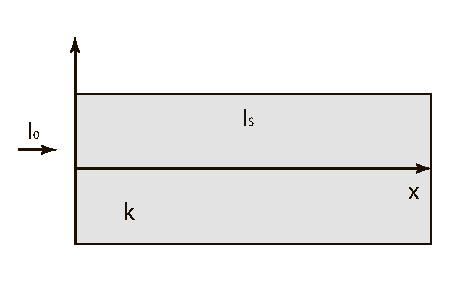
\includegraphics[width=.4\textwidth]{08_01}
  \vspace{-1.5em}
\end{figure}

Изменение интенсивности света по мере прохождения им расстояния \( x \):
\[
  dI = KI dx, \quad \text{тогда} \quad \der{I}{x} = KI.
\]

Учитывая, что \( K = K_0 / (1 + I / I_s) \), получим
\[
  \der{I}{x} = \frac{K_0 I}{1 + I / I_s}, \quad
    \frac{dI}{I} \left( 1 + \frac{I}{I_s} \right) = K_0\,dx.
\]
Интегрируя с учетом граничных условий, получим уравнение
\[
  \ln\frac{I}{I_0} + \frac{I}{I_s} - \frac{I_0}{I_s} = K_0 x, \text{ или }
    \ln\frac{I}{I_0} = f(K_0 x)
\]

\begin{figure}[h!]
    \center
    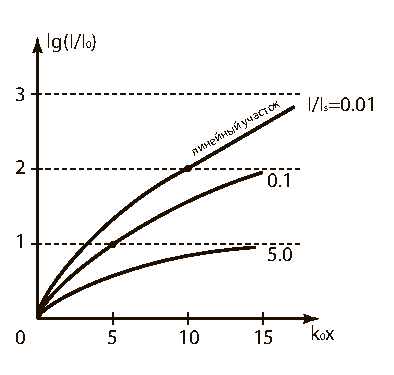
\includegraphics[width=.4\textwidth]{08_02}
\end{figure}

При малых уровнях интенсивности, когда \( I \ll I_s \) или \( I_0 \ll I_s \),
вынужденное излучение не влияет на концентрацию частиц в возбужденном
состоянии. Тогда \( I(x) = I_0\exp(K_0 x) \).

При \( I \gg I_s \): \( \D I / \D x \simeq I_s K_0 \).
В этом случае практически вся энергия возбужденной среды переходит в энергию
когерентного излучения. Скорость роста интенсивности стремится к постоянной
величине
\[
    I_s K_0 = \frac{h\nu\sigma N}{2\sigma\tau} = \frac{h\nu N}{2\tau} = \const.
\]

\subquestion{Нерезонансные потери в активной среде}

\begin{enumerate}
  \item Дифракционные.
    \begin{figure}[h!]
      \center
      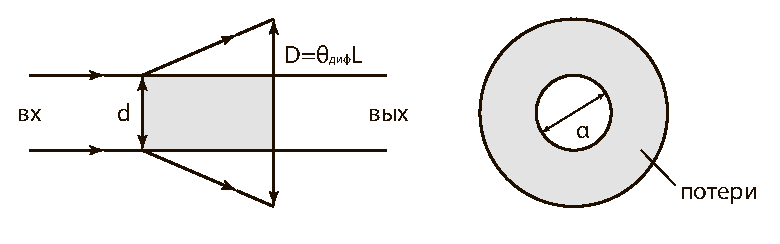
\includegraphics[width=.55\textwidth]{08_03}
    \end{figure}
    \[
      \vartheta_\text{диф} = 1.22\frac{\lambda}{d}; \quad
        \eta_\text{диф} = (90\ldots99)\%
    \]
  \item На оптических элементах (многопроходный усилитель).
    \begin{figure}[h!]
      \center
      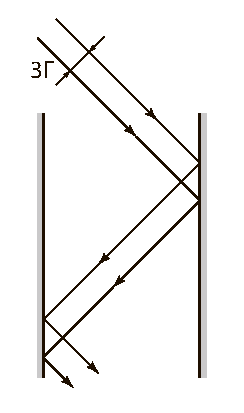
\includegraphics[width=.25\textwidth]{08_04}
    \end{figure}
    \[
      \eta_\text{опт} \approx 99\%
    \]
  \item На неоднородностях активной среды. \\
    Оптические неоднородности связаны с неоднородностью плотности среды,
    связанной с неоднородностью температуры, механического напряжения и т.~п.
\end{enumerate}
